\documentclass[a4paper]{article}

\usepackage[english]{babel}
\usepackage{amsmath}
\usepackage{graphicx}
\usepackage[latin1]{inputenc}
\usepackage[T1]{fontenc}
\usepackage{listings}
\usepackage{xcolor}
\usepackage{eso-pic}
\usepackage{mathrsfs}
\usepackage{url}
\usepackage{amssymb}
\usepackage{multirow}
\usepackage{hyperref}
\usepackage{caption}
\usepackage{siunitx}
\usepackage{booktabs}
\usepackage{hhline}

% packages [additional]
\usepackage{bbm}
\usepackage{setspace}
\usepackage{parskip}
\usepackage[margin=3cm]{geometry}

\title{Statistical Programming Languages: R. \\ Seminar - Group Project Report at the \\
Ladislaus von Bortkiewicz Chair of Statistics \\
Humboldt-University Berlin \\ \emph{Stock price drivers of oil and gas companies from the U.S.}}

\author{Marcus Goossens, Tim Halbmann \\ Antton Haramboure, Fabian Salger}

\newcommand{\qletz}{\raisebox{-1pt}{
\includegraphics[scale=0.15]{qletlogo}}}

\setlength{\parindent}{0cm}
\onehalfspacing
\newcommand*{\skippingparagraph}{\par\vspace{\baselineskip}}

\begin{document}

\maketitle

\begin{center}

\includegraphics{hulogo.pdf}\\[0.75cm]
\end{center}

\newpage

\tableofcontents

\newpage

\section{Introduction}

Our research project strives for robust panel data regression results regarding the non-renewable energy sector in the United States. Close to recent research on the subject, we aim at finding the main drivers of stock prices for large companies within the oil and gas producing industry. We therefore take 7 oil/gas firms for which we consistently find quarterly data for the last ten years, thereby focusing on balance sheet and market data. Apart from that, we looked at two utility companies. However, the latter ones have not been included in the panel data regressions that follow unless explicitly stated.

\begin{table}[ht]
\centering
\begin{tabular}{rl}
\hline
\hline
\multicolumn{2}{c}{Company}\\
\hline
$1.$ & Chevron  \\ 
$2.$ & Exxon Mobil  \\ 
$3.$ & Apache  \\ 
$4.$ & Hess Corp \\ 
$5.$ & Occidental Petrolium  \\ 
$6.$ & Murphy Oil  \\
$7.$ & CPEnergy$^{1}$ \\
$8.$ & PGE Corp$^{1}$ \\
$9.$ & Williams Cos, Inc.$^{2}$ \\
\hline
\hline
\multicolumn{2}{l}{$^{1}$electricity company} \\
\multicolumn{2}{l}{$^{2}$EDA-Case}
\end{tabular}
\label{}
\caption{Sample Companies} 
\end{table}

Possible drivers of stock prices can be common factors such as market returns, gas and oil prices and company-specific factors such as net income, leverage ratio, company size and the companies' respective financial market valuation. In order to get robust results, we transform our data to account for issues such as non-stationarity and test our regressions for serial correlation and heteroskedasticity.

Our analysis shows that problems like non-stationarity are present in our panel data and can partially be solved through transformations. The regression results seem to confirm former research that stock prices are driven by common and company-specific factors, leading to the conclusion that the energy market is not fully informationally efficient.

\section{Data Transformation Procedures}

In line with Bianconi and Yoshino (2014), we apply the data transformations as indicated in table 2 on our set of variables.

\begin{table}[ht]
\centering
\begin{tabular}{l|l|l}
\hline
\hline
\multicolumn{1}{c|}{Log Return} & \multicolumn{1}{c|}{Z-Score / Standardization} & \multicolumn{1}{c}{Log} \\
\hline
Stock & NI & A.MCAP$^{1}$ \\ 
Oil &BVE.MCAP &  D.MCAP\\ 
Gas& & \\ 
Market$^{2}$& &\\ 
EX$^{3}$& & \\ 
\hline
\hline
\multicolumn{3}{l}{\footnotesize $^{1}$ due to collinearity issues, 'A.MCAP' excluded in subsequent analyses} \\
\multicolumn{3}{l}{\footnotesize $^{2}$ Dow Jones Industrial Average (DJI)} \\
\multicolumn{3}{l}{\footnotesize $^{3}$ USD w.r.t. EUR, GBP, [...]}
\end{tabular}
\label{}
\caption{Variables by Transformation Mode}
\end{table}

The Market excess return was obtained in the following way: $ln(\frac{Market_{t}}{Market_{t-1}})-r^{f}_{t}$. The risk-free rate was defined to be the interest rate of three-month U.S. Treasury bill (denominated in US dollars). Expressing the companies' stock prices and the common factor prices as log-returns is helpful for the following reasons.

An absolute change in, for instance a rise of the oil price, of US\$10 is likely to have a substantially different impact given that, at the beginning of the quarter oil was trading at US\$30 or US\$100. Apart from that, having specified both the dependent and the independent variable as log returns, one could interpret a $\Delta xi = 1 \%$ in the explanatory variable as following marginal effect: $\Delta Y=\Delta xi \beta_i = \beta_i\%$.

Yet since our sample is rather small and fails to adequately fulfil several econometric requirements, we constrain to qualitatively interpreting our panel data regression results. 

Applying a standardization procedure to Net Income (NI) as well as Book Value of Equity over Market Capitalization (BVE.MCAP) turns out to be helpful because the companies in our sample are of different size. This means that a US\$1 million increase of net income can have different implications for Apache Crop than for Exxon Mobil. By standardizing Net Income, we can make the profitability variations of the firms comparable as it is more likely that a Net Income increase of one standard deviation within a quarter has a similar impact on the quarterly stock return for all companies. 

A similar reasoning applies when it comes to BVE.MCAP: due to (historically) being involved in different sub-sectors of the oil and gas industry, a firm might carry more or less assets evaluated at less than market value on its balance sheet. Apart from that, the firm might also possess intangible assets which value is incorporated in the market value, but not the book value. By standardizing this variable, analyzing the impact of its variation becomes more comparable across companies. 
The variables A.MCAP and D.MCAP transformed by taking the log because these two variables are likely to be log-normally distributed. Note that the application of a log also simplifies the interpretation of the marginal effects. A similar reasoning as in the log returns case applies. 

Note that, by applying the log returns on quarterly data, we approximate the percentage change in the respective variables, which would actually be given by: $\Delta(Oil_{t,t-1})\% = \frac{Oil_t - Oil_{t-1}}{Oil_{t-1}} \approx ln (\frac{Oil_t}{Oil_{t-1}})$. This approximation holds well as long as the \%-variation of the variable is not too large. Considering the mean log returns of stock price, oil price, gas price and exchange rates, this approximation appears to be valid, with respective means ranging from $-0.03$ to $0.01$. Yet when considering the highest and the lowest log returns of the variables, this approximation is not accurate anymore because quarterly stock price variations range between $-75\%$ and $+73\%$. The same applies for oil and gas price changes. For carrying out quarterly-based analyses, it would therefore have been more adequate to compute discrete quarterly returns for using them in subsequent econometric analyses. 

In the case of Bianconi and Yoshino, who based their investigation daily returns, the application of log-returns is likely to be less problematic because stock and commodity priced do not vary to such a large extent as in our case on a daily basis.\footnote{Using the log return approximation instead of the more accurate discrete version is unlikely to trigger fatal effects such as estimation coefficient sign reversals and similar severe consequences}  

\emph{Stationarity Matters}

The issue of spurious regression (triggering a nonsense correlation) can arise when one tries to estimate the relationship between nonstationary explanatory variables and a (also nonstationary) dependent variable of a time series resorting to OLS. This is due to the fact that
\emph{"[...]in a time series spurious regression of $Y_t$ on $X_t$, the limit of the OLS estimator is a non-degenerate random variable being a function of Brownian Motions" Phillips (1986)},
rather than an estimator of the beta of the underlying time series under investigation. 

\emph{Non-Stationarity in Panel Data}

In light of the severe impact of a spurious regression, we checked the adequacy of the panel data analysis tools we resorted to in our analysis. Phillips and Moon (2001) found that independent cross sectional data (i.e. that panel data includes different individuals) adds information, improves the overall signal from the data at hand and might mitigate the problem. This reasoning applies given that both panel data dimensions (number of individuals, N, and time lapses, T) are large, not to forget the independence assumption regarding the draws. The latter might not hold in our analysis because all companies being part of the sample are US companies. Apart from that, the panel we used included nine companies and 78 quarters (from Q3-1996 to Q4-2015) and is thereby relatively small. For the reasons mentioned, the potential existence of non-stationary variables in our panel has been under scrutiny. 

The analysis of Bianconi and Yoshino (2014) serves as a central reference point of this seminar project. Their research sample consists of 64 companies from 26 countries and looks at the time frame lasting from July 15, 2003 until August 14, 2012 on a daily basis (T = 3,381 days). Several companies at their consideration were not part of the sample for the full time period. However, they were still left with about 115,000 observations. Non-stationarity might therefore be less of an issue affecting their estimations. 

\emph{Sample Stationarity Checks}

In order to detect whether the (non-) transformed data set has a unit root, hinting at nonstationarity, the Levin-Lin-Chu Unit Root test called by the function purtest() being part of the plm package was implemented. The null hypothesis of this test is that the underlying data exhibits nonstationary patterns. 

Since the Levin-Lin-Chu tests considers the whole dataset, but not the individual variables having been transformed in different fashions, we resorted to the Augmented Dickey Fuller Test (adf.test()) as well as the KPSS test checking the stationarity for each variable by company. Note that the null hypothesis of the ADF-test is that the underlying variable contains a unit root (hinting at nonstationarity) whereas the null of the KPSS-test is that the given variable is (trend) stationary. The significance level for both tests was set at 10\%. 

Nontransformed variables

The Levin-Lin-Chu Unit Root Test clearly states that a unit root is present in the given panel data set. 

\begin{table}[ht] 
\centering
\begin{tabular}{l|l|ll}
\hline
\hline
\multicolumn{1}{c|}{Variables} & \multicolumn{1}{c|}{ADF-Testresult} & \multicolumn{1}{c}{KPSS-Testresult} \\
\hline
Stock & n.st. & n. (trend) st. \\ 
Oil & n.st. &  n. (trend) st. \\ 
Gas & n.st. & n. (trend) st. \\ 
Market & n.st. & n. (trend) st. \\ 
EURUSD & n.st. & n. (trend) st. \\ 
\hline
\hline
\end{tabular}
\label{}
\caption{Stationarity of common factors} 
\end{table}

\begin{table}[ht] 
\centering
\begin{tabular}{l| l| l| l| l| l}
\hline
\hline
\multicolumn{1}{c|}{Firm} & \multicolumn{1}{c|}{Stock Price} & \multicolumn{1}{c|}{A.MCAP} & \multicolumn{1}{c|}{BVE.MCAP} & \multicolumn{1}{c|}{D.MCAP} & \multicolumn{1}{c}{NI} \\
\hline
Exxon Mobil & n.st. & n.st. & n.st. & n.st. & n.st. \\ 
Apache & n.st. & n.st. & n.st. & n.st. & n.st. \\ 
CPEnergy & n.st. & n.st. & n.st. & n.st. & st. \\ 
Chevron & n.st. & n.st. & n.st. & n.st. & n.st. \\ 
Hess-Corp & n.st. & n.st. & n.st. & critical a[0.1,0.2] & n.st. \\
Murphy Oil & n.st. & n.st. & n.st. & n.st. & n.st. \\ 
Occidental & n.st. & n.st. & n.st. & n.st. & n.st. \\ 
PGE Corp & n.st. & n.st. & st. & n.st. & st. \\ 
Williams & n.st. & n.st. & critical a[0.1,0.2] & n.st. & critical a[0.1,0.2] \\ 
\hline
\hline
\end{tabular}
\label{}
\caption{Stationarity of enterprise-specific factors} 
\end{table}

The tests clearly show that the non-transformed panel data is non-stationary. Therefore, the variables were transformed in the following way. Yet only one out of the three transformations applied by Bianconi and Yoshino in their publication has actually the potential to tackle the issue of non-stationarity in our sample.

\begin{table}[ht]
\centering
\begin{tabular}{l|l|l}
\hline
\hline
\multicolumn{1}{c|}{Variables} & \multicolumn{1}{c|}{Transformation Applied} & \multicolumn{1}{c}{Stationarity rendering-potential} \\
\hline
Stock Price & Log return & Yes. The variables are detrended \\
Oil Price &  &  \\ 
Gas Price &  & \\ 
Market$^{1}$&  &\\
\hline
Net Income (NI) & Standardization / Z-Score & no $^{2}$ \\
BE.MCAP &  & \\
\hline
A.MCAP & Log & no \\
D.MCAP &  & \\
\hline
\hline
\multicolumn{3}{l}{\footnotesize$^{1}$Dow Jones Industrial Average (DJI)} \\
\multicolumn{3}{l}{\footnotesize$^{2}$\begin{tabular}[t]{@{}l@{}}De-meaning and then scaling variables makes variations across \\ companies more comparable, yet is unlikely to provide non-stationarity\end{tabular}}
\end{tabular}
\label{}
\caption{Variables by Transformation Mode} 
\end{table}

\emph{Transformed variables}

The Levin-Lin-Chu Unit Root Test states that no unit root is present in the transformed panel data set. The p-value obtained is rather low: $p=2.2e^{-16}$ Yet since different transformations have been applied to different variables, it is worthwhile to check if the individual transformed variables turn out to be stationary.

\begin{table}[ht]
\label{}
\centering
\begin{tabular}{l|l|l}
\hline
\hline
\multicolumn{1}{c|}{Variable} & \multicolumn{1}{c|}{ADF-Testresult} & \multicolumn{1}{c}{KPSS-Testresult} \\
\hline
Oil return & st.& (trend) st. \\ 
Gas return & st. & (trend) st. \\ 
Market excess return& st. & (trend) st. \\ 
EURUSD return & st. & n. (trend) st. \\
\hline
\hline
\end{tabular}
\caption{Stationarity of Common Factors (Oil Price, Gas Price, Market)} 
\end{table}
This seems to hold for the common factors of the sample. 

\emph{Stationarity of enterprise-specific factors}

\begin{table}[ht] 
\label{}
\centering
\begin{tabular}{l| l| l| l| l| l}
\hline
\hline
\multicolumn{1}{c|}{Company} & \multicolumn{1}{c|}{Stock Return} & \multicolumn{1}{c|}{A.MCAP} & \multicolumn{1}{c|}{BVE.MCAP} & \multicolumn{1}{c|}{D.MCAP} & \multicolumn{1}{c}{NI} \\
\hline
Exxon Mobil & st. & n.st. & n.st. & n.st. & n.st. \\ 
Apache & st. & n.st. & n.st. & n.st. & n.st. \\ 
CPEnergy & st. & n.st. & n.st. & n.st. & st. \\ 
Chevron & st. & st. & n.st. & n.st. & n.st. \\ 
Hess-Corp & st. & n.st. & n.st. & n.st. & n.st. \\
Murphy Oil & st. & n.st. & n.st. & n.st. & n.st. \\ 
Occidental & st. & n.st. & n.st. & n.st. & n.st. \\ 
PGE Corp & st. & n.st. & st. & n.st. & st. \\ 
Williams & st. & n.st. & critical a[0.1,0.2] & n.st. & critical a[0.1,0.2] \\ 
\hline
\hline
\end{tabular}
\caption{Stationarity of enterprise-specific factors} 
\end{table}
As expected when mentioning the variable transformations applied, it is of hardly any surprise that the enterprise-specific variables remain nonstationary after their respective transformation\footnote{Applying the KPSS-test instead of the ADF-test, we come to the same conclusion}. 

\emph{Conclusion of Stationarity Tests}

One has to bear the results of the applied stationarity checks into account when it comes to the interpretation of the regression results. Since the sample used for this analysis may be too small in both dimensions, and likely too homogeneous as well, non-stationarity of the enterprise-specific variables is problematic. For previously stated reasons, we therefore always compared our findings with the ones of Bianconi and Yoshino (2014).
 
\emph{Application of the ADF and KPSS test by both company-specific variables and company}

Note that since the KPSS test results retrieval is, apart from the test itself, similar to the procedures for obtaining the ADF-Test results, only the latter one is covered here. The tests are carried out in the VarTransStation quantlet. 

The test result retrieval consists of three parts: 2 functions followed by the application of the second function on the adequate subset of the data, the specific factors. The first function, 'stattestFUN', (lines 63 to 75, performs the ADF-test on an input vector x and returns a character string stationary / not stationary response. Note that this function is called within the second function. 

\begin{small}
\begin{lstlisting}
# Stationarity Test - ADF Test
stattestFUN = function(x){
    test       = adf.test(x, alternative = "stationary")
    testresult = test$p.value
    testresult = round(testresult, digits = 2)
    if(testresult < 0.1){
        ReturnResult = "stationary"
    }else if(testresult > 0.1 & testresult < 0.2){
        ReturnResult = "Critical a[0.1,0.2]" 
    }else{
        ReturnResult ="not_stationary"
    }
}
\end{lstlisting}
\end{small}
\begin{center}
Quantlet 1 - Variable Transformation: Lines 63-75 \href{https://github.com/Fabian-HC/SPL-OilUS/blob/master/VarTransformSta/VarTransStation.R}{\protect \qletz}\\[0.5cm]
\end{center}

The second function, called ADFEntSpecTestFun, specified in lines 103 to 112, performs several steps to then return a table detailing the stationarity test results for all company-specific variables for each company. 

\begin{small}
\begin{lstlisting}
ADFEntSpecTestFun = function(x){
    ADFTest           = aggregate(x, by = list(data$Company), 
                                  FUN = stattestFUN, simplify = FALSE)
  
    ADFTest           = ADFTest[,-1]
    ADFTest           = do.call("rbind", lapply(ADFTest, as.data.frame))
    colnames(ADFTest) = levels(data$Company)
    ADFTest           = as.data.frame(t(ADFTest))
  return(ADFTest)
}
\end{lstlisting}
\end{small}
\begin{center}
Quantlet 1 - Variable Transformation: Lines 103-112 \href{https://github.com/Fabian-HC/SPL-OilUS/blob/master/VarTransformSta/VarTransStation.R}{\protect \qletz}\\[0.5cm]
\end{center}

The most crucial and intriguing step is the first one: The aggregate function, which is also used in other parts of this seminar project, retrieves variable (j)-specific information for a specific company (i). One can consider it as a successful attempt to run an apply-function on the company-specific subsection of a column! When specifying 'by', we manage to tell R to subdivide the variable under consideration by company. Simplify has to be set to FALSE as R, according to some mechanisms at hand, which we do not want to apply here, tries to simplify the output and coerce it into a matrix.

As the aggregate function in this case returns a list\footnote{from which we remove the first column not being of interest as it merely specifies item names}, one has to transform the list within several steps into a correctly labelled data frame. For this purpose, one calls the 'rbind' function in line 108 and applies it to every element contained in the list 'ADFTest'. In the next step, the company names are set to be the column names. As a last step, the ADFTest data frame is turned upside down (the matrix transformation is applied to it) to then eventually yield a data frame in the presentable desired format.

We specified the two functions in the function section of the code and therefore do not obstruct the view when looking at the functions and transformations applied on the data itself.

In the third step, the 'ADFEntSpecTestFun' is called in the code. The adequate, company-specific variables data section is then fed into the function. It provides us with the data frame containing the "responses" of the ADF test for the company specific variables by company. This one is then stored in an auxiliary data frame which is then passed on to the write.csv2() as well as the print.xtable() command in order to export the tabular representation of the ADF-Test results into a Excel-readable CSV-file as well as a \LaTeX\ code. 

\section{Exploratory Data Analysis}

Despite all advances and developments concerning panel data regression, exploratory data analysis is nevertheless a necessary initial step to be carried out. 

First of all, we have the opportunity to detect first hints whether, apart from the hypothesis postulating how the common factors (Oil price, gas price, stock market developments) and enterprise-specific variables can affect stock returns of US oil companies, there might be other factors at work as well. For example, if a company is affected by financial distress, company-specific variables, such as leverage, can have a different impact than if the firm was financially sound. A more detailed discussion follows. On top of that, we can check whether certain assumptions that have to be satisfied by the empirical models used, indeed hold (to a sufficiently large extent) in our data. 

\emph{Summary statistics and Graphical Analysis for pre-transformed variables}

In particular with respect to the enterprise-specific variables, summary statistics help us to get an overview regarding our companies and, in particular, their financial health throughout our sample period\footnote{This analysis is carried out based on the non-transformed variables as a first step, in order to provide an overview}. 

\begin{table}[ht]
\centering
\begin{tabular}{l|r|r|r|r}
\hline
\hline
\multicolumn{1}{c|}{Variable} & \multicolumn{1}{c|}{mean} & \multicolumn{1}{c|}{sd} & \multicolumn{1}{c|}{min} & \multicolumn{1}{c}{max} \\
\hline
Stock & 43.13 & 21.65 & 12.51 & 92.34 \\ 
BVE.MCAP & 0.59 & 0.24 & 0.27 & 1.65 \\ 
D.MCAP & 97.29 & 56.82 & 37.68 & 310.68 \\ 
NI & 1186.45 & 1200.02 & -2937.10 & 4056.13\\ 
\hline
\hline
\end{tabular}
\label{}
\caption{Mean values of enterprise-specific variables}  
\end{table}

From this table, we can already extract some relevant pieces of information. According to our sample, the representative US oil and gas company has an unweighted mean leverage ratio of about 97\% \footnote{Leverage definition used: Debt over Market value of equity (Market value of equity = share price * shares outstanding} - therefore, on average, the companies in our sample are 50\% debt financed. The average leverage maximum equalled 310\% implying that the firm was about $\frac{3}{4}$ debt financed at some point. As leverage definition, we use debt over the market value of equity, where the market value of equity is the product of share price multiplied with the total number of shares outstanding.

The average book value of equity over market value of equity was 0.59, or 59\%. This implies that the market values a company by $\frac{1}{0.59} - 1=169.49\%-1 = 69.49\%$ more than its book value. Thus, market participants price in, on average, an equity growth potential equalling in total about 70\%. Another potential reason could be that the average firm is carrying assets on its balance sheet at less than market value or is omitting other assets like brand assets and knowledge assets. Historical cost accounting and the immediate expensing of R\&D (Research and Development related costs) and expenditures on brand creation produce balance sheets that are likely to be below market value.

All companies, except for Exxon Mobil and Occidental Petroleum, have a maximum book value of equity over market value of equity-ratio above one at some moment in our sample period. A ratio above one indicates that a stock sells for less than book value meaning that the return on equity is less than the required rate of return for an equally risky firm by market participants. This can be interpreted in the following way: Stock market participants thought, during the hardest times of a company, that it would not grow, but shrink and that, in fact, its future (free) cash flows to equity would be of less value than the book value of equity.

By deriving summary statistics company wise, one can detect outliers among the companies. For instance: Center Point Energy (CPEnergy) and PG\&E Corp exhibit sky-high leverage ratios. By taking into account the development of their leverage ratios over time using the plots and cross-checking resorting to past financial news and company information, one finds that PG\&E Corp went almost bankrupt at the beginning of the 2000s decade. During this time period, oil prices were comparatively low, but stable. The stock market still had to adjust to the Dotcom-bubble, yet that is unlikely to trigger an almost bankruptcy event of a non-renewable energy sector firm. This piece of information is insofar relevant that the econometric models used later on were not established for analysing the development of the stock return of oil firms during  financial distress situations, but rather the impact of common market factors and enterprise specific factors (under normal financial conditions). Note that, as PG\&E Corp. is a company producing electricity and being active in the gas sector, it will not be included in several subsequent regression analyses because for those our company group of interest were oil and gas exploring and extracting companies of the United States. 

A somewhat similar argument holds for Center Point Energy Inc. This company was split up in 2003 as the state of Texas deregulated its utility and electricity market. In this context, summary statistics and time series graph analysis turned out to be a helpful tool for analyzing differences between the companies and narrowing the sample down to the industry which is at the center of interest of this analysis.

Yet also among the oil companies we observe financial distress events. This is the case for Williams Cos Inc. In 2002, the company was at the margin of bankruptcy as well. One cause was that energy companies in general came under pressure in the wake of the Enron scandal casting doubts on the financial health of other companies, too. Eventually, Warren Buffet provided the company with a high-interest loan in order to avoid bankruptcy.

\begin{figure}[h]
\begin{center}
\vspace{-2cm}
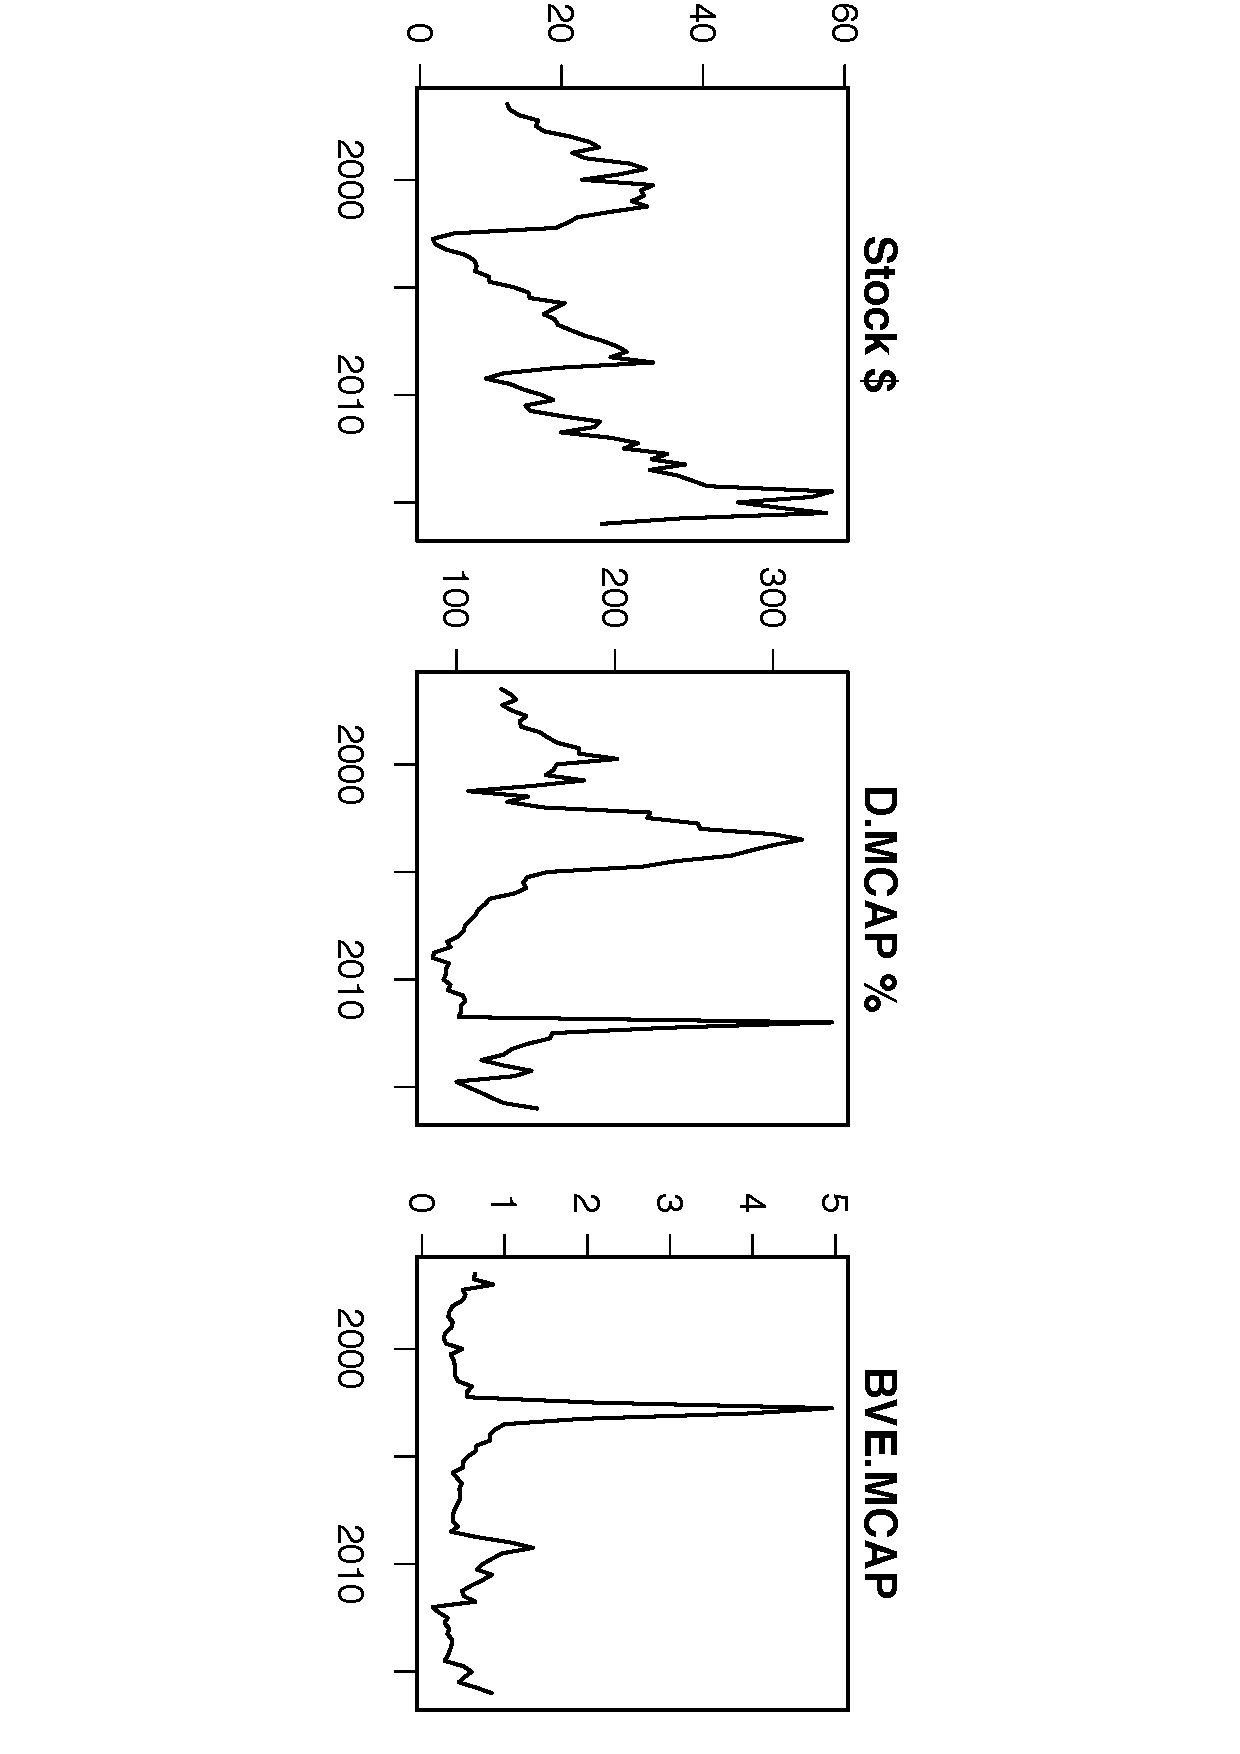
\includegraphics[scale=0.5,angle=90]{C9_Williams_Report.pdf}
\vspace{-2.8cm}
\label{}
\caption{Financial Distress Case of Williams Cos Inc.}
\end{center}
\end{figure}

All things considered, one can hold that the exploratory data analysis already helps to detect events triggering consequences that might be out of the scope of the empirical models applied. One would now have to decide whether to

\begin{itemize}
  \item[a.]  exclude the company-specific periods of financial distress or other extreme situations,
  \item[b.]  exclude the company affected altogether, or
  \item[c.]  keep the company in the sample without even excluding the exceptional time periods.
\end{itemize}

The sample at hand features $N=9$ companies and includes $T=78$ periods. For this reason, the fact that three out of all companies had to face financial difficulties during the sampling period might alter the regression results obtained. One reason can be that, at the margin of bankruptcy, companies, crudely speaking, run out of equity. Therefore, the leverage ratio (indicating excessive indebtedness in such a case) and the book value of equity by market value of equity ratio (BVA.MCAP) skyrocket. The substantial increase in those explanatory variables comes in combination with a substantial drop in stock price. So the interrelation between an increase in the two explanatory variables mentioned and the stock return is negative and close to mechanic in this particular situation. 

Yet this might not be the case given that the company is financially sound. In such a situation, a higher leverage ratio (D.MCAP) leads to a higher stock return in expectation because: 

\begin{enumerate}
\item	The ratio $\frac{Net Income}{Equity}$ assumes a higher value;
\item In fact, equity holders require a higher expected stock return in order to be compensated for the additional risk arising from leverage
\end{enumerate}

Apart from that, levering up also increases the variability of the return on equity / the stock return. Moreover, agency costs and benefits of leverage and tax implications also have an impact on how leverage affects the stock returns. The topic is covered by Berk/DeMarzo in their Corporate Finance (3rd edition) text book.

Considering all these factors, the impact of more or less leverage cannot be unambiguously determined beforehand. Note that the linear specification applied in the regression model and in the paper of Bianconi/Yoshino (2014) does not take potential non-linear impacts of leverage into account, which may have less impact on the results of their larger sample.

\begin{figure}[ht]
\begin{center}
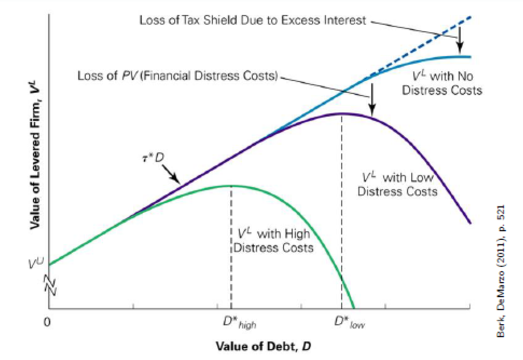
\includegraphics[scale=1]{cofi-berk-demarzo.pdf}\\
\label{}
\caption{Financial Distress may exceed the model scope [directly from Berk, DeMarzo (2011), p.521]}
\end{center}
\end{figure}

Considering the research by Bianconi/Yoshino (2014) mentioned, and on which our seminar project is based, the following differences were cautiously considered:

\begin{enumerate}
\item Since Bianconi/Yoshino decided to consider daily variations in common factors and company-specific variables, the financial distress period of the three companies mentioned might already have a minor impact as there are more time lapses within which the company is financially sound and the driving forces specified in the empirical models considered apply. 
\item For their empirical analysis, the two include not only 9, but 56 companies in their sample. Given that none of the additional companies included faced a financial distress situation, their estimates have not been significantly driven by the distress events of the three companies in this sample.
\end{enumerate}

\emph{Retrieval of graphs and company-specific summary statistics}

As previously mentioned, company-specific summary statistics helped us a lot in the exploratory data analysis. The 'describeBy' command being part of R's 'psych-package' has turned out to be a rather handy tool.

Lines 46 to 48

Since by is already contained in the command name, it is clear that this command can provide us summary statistics differentiating by company: One simply has to specify 'group = "Company"' (or another variable name if the differentiation is to occur with respect to another variable (see line 47). 'describeBy' also offers the optional feature of delivering its output as a matrix rather than a list. This is helpful as one normally represents summary statistics later on in exported \LaTeX\ or Excel tables, which in turn can only be obtained from R via data frames or matrices. 

For the given purpose, it was necessary to set 'trim' equal to zero. If trim was, for instance, 0.1, R would have cut off the upper and the lower 10\% quantile of the given variable of company 'j'. Yet since minima and maxima were of interest, this value is set to zero. The option 'type' specifies the manner with which skewness- and kurtosis-values are computed. Here it is set to 1 because this type computes the values presuming that the data set contains the whole population. This is insofar true here as there is data for all quarters of variable 'j' of company 'i'. In this sense, no selection of quarters was randomly extracted. 

Remaining lines: 49 to 58

These lines get the matrix delivered by the 'describeBy' command into shape. In line 50 and 51, several summary statistics and one variable specifying item numbers are removed. In line 52. The matrix is ordered so that at first all variables of the first sample company show up, then the second ones, etc. In a next step, in line 53 and 54, the variables (vars), being numbers so far, are converted into factor variables to then replace the numbers by the adequate variable names. Lines 55 to 58 are cosmetic adjustments to the matrix which is then put out. 

\begin{small}
\begin{lstlisting}
# Derive company-specific variables' summary statistics by company
SumSpecFun = function(data){
    SumSpec = describeBy(data[,2:7], group = "Company", 
                         mat = TRUE, digits = 2, trim = 0, type = 1)
  # Extracting summary statistics of interest and cosmetic adjustments
    SumSpec			= SumSpec[-c(1:9),]
    SumSpec			= SumSpec[,-c(4,7:9,12:15)]
    SumSpec			= SumSpec[order(SumSpec$group1, SumSpec$vars),]
    SumSpec$vars		= factor(SumSpec$vars)
    levels(SumSpec$vars)	= colnames(data[,3:7])
    SumSpec			= SumSpec[,-1]
    rownames(SumSpec)		= NULL
    return(SumSpec)
}
\end{lstlisting}
\end{small}
\begin{center}
Quantlet 2 - EDA: Lines 45 to 58 \href{https://github.com/Fabian-HC/SPL-OilUS/blob/master/EDA_PanDat/EDA_PanDat.R}{\protect \qletz}\\[0.5cm]
\end{center}

This function is eventually applied to a given data frame in line 94 as well as line 129 of this the EDA PanDat.R quantlet.

\section{Econometric Approach}

Since we are dealing with panel data that allows us to work with data observed on cross-sections of units (companies) and over time, we have to cope with the problem of unobserved heterogeneity across companies. To deal with that issue, we use the unobserved effects model that models individual heterogeneity by introducing an error term with two separate components:

$y_{it} = \alpha + \beta^{T} x_{it} + \mu_i + \epsilon_{it}$

The error component $\mu_i$ is specific to the individual and does not change over time (individual effects) whereas the idiosyncratic error $\epsilon_{it}$ is assumed to be independent of both the regressors $x_{it}$ and the individual error component $\mu_i$.

Dependent on whether the individual component is correlated with or independent of the regressors, the appropriate estimation method will be chosen. In case of correlation, the fixed effects model will be applied, the random effects model otherwise. 

In case of individual homogeneity, meaning that $\alpha_{it}=\alpha$ and $\beta_{it}=\beta$, the resulting model would be pooling all the data across $i$ and $t$:

$y_{it}=\alpha+\beta^{T}x_{it}+u_{i}$

The individual component would be missing as well. 
If one wants to allow for the idiosyncratic error $\epsilon_{it}$ to be arbitrarily heteroskedastic and serially correlated over time, a GLS model has to be applied. 

In order to find an appropriate estimator, we consider the following steps:
\begin{itemize}
\item
test for poolabilty, i.e. the hypothesis that the same coefficients apply across all individuals
\item
test for the presence of unobserved effects
\item
Hausman test for the choice between fixed and random effects model
\item
Robust diagnostics, i.e. test for heteroskedasticity and serial correlation in idiosyncratic errors
\end{itemize}

\section{Empirical Results}

From a theoretical perspective, stock prices can be driven by many factors. According to the Capital Asset Pricing Model (CAPM), those factors can be subdivided into systematic and non-systematic (idiosyncratic) risk components. CAPM theory postulates that only systematic risk factors such as the market portfolio excess return are priced in stock returns whereas non-systematic factors do not drive stock returns. These idiosyncratic risk components refer to company-specific characteristics, e.g. net income or leverage ratio, and therefore are diversified away by forming large portfolios so that investors will not be compensated for company-specific risks.

One crucial assumption of the CAPM is that capital markets are efficient meaning that information asymmetries do not exist and therefore do not pose a market friction. This stylized case of fully efficient markets is not very likely do hold in reality leading to the conclusion that empirical results should reflect an exposure of stock prices to both, systematic and non-systematic risk factors and our main objective is to measure and price those risks.

\subsection{Hypotheses}

H1: Oil and gas price returns have a robust - i.e. statistically significant - positive effect on stock price returns because higher price returns indicate the presence of a profitable environment for oil companies that will result in a higher cash flow to the firm, thereby increasing its equity value.

H2: Since energy consumption is related to the overall economic situation, the exposure of stock price returns to the U.S. Dowjones Industrials market premium returns is robustly priced and positive.

H3: Non-systematic risk factors such as company value and net income are important factors that are robustly priced.

\subsection{Correlation Coefficients}

By looking at the unconditioned correlation coefficients of the variables, one can already get a first impression of how the independent variables correlate with the stock returns of the seven oil firms but also correlations among themselves.

\begin{table}[ht]
\begin{tabular}{l|r|r|r|r|r|r|r}
\hline
\hline
\multicolumn{1}{c|}{Variable} & \multicolumn{1}{c|}{Stock} & \multicolumn{1}{c|}{A.MCAP} & \multicolumn{1}{c|}{BVE.MCAP} & \multicolumn{1}{c|}{D.MCAP} & \multicolumn{1}{c|}{NI} & \multicolumn{1}{c|}{Oil} & \multicolumn{1}{c}{Gas} \\
\hline
Stock &  1.00  &  &  &  &  &  &  \\ 
  A.MCAP & ***-0.24 &  1.00  &  &  &  &  &  \\ 
  BVE.MCAP & ***-0.34 & **0.58 &  1.00  &  &  &  &  \\ 
  D.MCAP & -0.01 & ***0.65 & -0.03  &  1.00  &  &  &  \\ 
  NI & ***0.15 & ***-0.18 & **-0.10  & ***-0.31 &  1.00  &  &  \\ 
  Oil & ***0.44 & **-0.10 & ***-0.22 &  0.03  & **0.11 &  1.00  &  \\ 
  Gas & ***0.27 & -0.04  & **-0.11  &  0.07  &  0.02  & ***0.36 &  1.00  \\ 
  Market & ***0.39 & -0.01  &  0.04  & -0.03  &  0.01  & ***0.12 & *0.08  \\ 
\hline
\hline
\end{tabular}
\label{}
\centering
\caption{Correlation matrix of all - idiosyncratic and common - factors}
\end{table}

At a first glance one recognizes that the common factors oil, gas and market return are positively correlated with stock returns, in support of our first two hypotheses. Note that these are all unconditional correlation coefficients such that the power of interpretation is limited. The third hypothesis is being supported by the coefficients for net income (NI) and company value (BVE.MCAP). 

When looking at the proxy for company size (A.MCAP) one can observe that the variable is highly correlated with BVE.MCAP and the leverage ratio (D.MCAP). This observation leads to the conclusion that A.MCAP might not be suited as a regressor because the independent variables are assumed to be uncorrelated. We rocognize that the assumption of no perfect multicollinearity is crucial when it comes to Panel Data Regression Models, such as POLS, FE, and RE.

By looking at the unconditioned correlation coefficients of the variables\footnote{myowelt.blogspot.de (2011) [last viewed online on August 13, 2016]}, one can already get a first impression of how the independent variables correlate with the stock returns of the seven oil firms but also correlations among themselves.

At a first glance one recognizes that the common factors oil, gas and market return are positively correlated with stock returns, in support of our first two hypotheses. The third hypothesis is being supported by the coefficients for net income (NI) and company value (BVE.MCAP). 

When looking at the proxy for company size (A.MCAP) one can observe that the variable is highly correlated with BVE.MCAP and the leverage ratio (D.MCAP). This observation leads to the conclusion that A.MCAP might not be suited as a regressor because independent variables are assumed to be uncorrelated.

A function is created in order to get a correlation coefficient table in \LaTeX\ that includes all variables and only displays the lower triangle of the symmetric matrix (including the diagonal). The function is structured as follows:

\begin{itemize}
\item
Lines 43-45:	First of all, x is defined as a matrix created from the given data set. R is defined as the extraction matrix of all correlation coefficients of the data set matrix R, and p is defined as the extraction matrix of the p-values.
\item
Line 48:		Defines the significance levels and returns a matrix with all stars by going through three ifelse functions for the p-value, starting with the lowest threshold. 
\item
Line 51:		Produces a matrix containing all coefficients rounded to two digits.
\item
Line 54:		Produces a symmetric matrix containing coefficients and their corresponding stars without spacing in between.
\item
Line 55:		Removes the N/A's from the diagonal.
\item
Lines 56-57:	Renaming rows and columns according to their variable names which get lost when building the new matrix.
\item
Lines 60-62:	Removing the upper triangle of the symmetric matrix while keeping the diagonal and returning a data frame.
\item
Line 65:		Removing last column because it does not contain any information.
\end{itemize}

\begin{small}
\begin{lstlisting}
# === Create unconditioned correlation matrix for variables ===
# Excluding variables that are not interesting
data2   = data[,c(3:10)]

# Create funtion for matrix
corrma  = function(x){ 
  require(Hmisc) 
  x     = as.matrix(x) 
  R     = rcorr(x)$r 
  p     = rcorr(x)$P 
  
  # Define notions for significance levels
  stars = ifelse(p < .01, "***", ifelse(p < .05, "** ", ifelse(p < .1, "* ", " ")))
  
  # Truncates matrix that holds the correlations to two decimal
  R     = format(round(cbind(rep(-1.11, ncol(x)), R), 2))[,-1] 
  
  # Build a new matrix that includes the correlations with their apropriate stars 
  Rnew            = matrix(paste(R, stars, sep=""), ncol=ncol(x)) 
  diag(Rnew)      = paste(diag(R), " ", sep="") 
  rownames(Rnew)  = colnames(x) 
  colnames(Rnew)  = paste(colnames(x), "", sep="") 
  
  # Remove upper triangle
  Rnew = as.matrix(Rnew)
  Rnew[upper.tri(Rnew, diag = FALSE)] = ""
  Rnew = as.data.frame(Rnew) 
  
  # Remove last column and return the matrix (which is now a data frame)
  Rnew = cbind(Rnew[1:length(Rnew)-1])
  return(Rnew) 
}

# Apply function and get otput
corrma(data2)
print(xtable(corrma(data2)), type = "latex", size = "tiny", file = "./corrma.txt")
\end{lstlisting}
\end{small}
\begin{center}
Quantlet 3 - Panel Data Analysis: Lines 36-71 \href{https://github.com/Fabian-HC/SPL-OilUS/blob/master/PanelDataAnalysis/PanelDataAnalysis.R}{\protect \qletz}\\[0.5cm]
\end{center}

\subsection{Panel Data Analysis}

\emph{Linear unobserved effects in the Panel Data Model}

The panel regression will look as follows\footnote{According to the pooltest, poolabilty is rejected} 

$R_{it} = \alpha + \beta_{1}NI_{it} + \beta_{2}BVE.MCAP_{it} + \beta_{3} D.MCAP_{it} + \beta_{4} Oil_{it} + \beta_{5} Gas_{it} + \beta_{6} Market_{it} + \mu_i + \epsilon_{it}$

The regression results for fixed and random effects look as follows, where significance levels are: p < 0.01, "***", p < 0.05, "** ", p < 0.1, "*"\footnote{significance levels are: p < 0.01, "***", p < 0.05, "** ", p < 0.1, "*" - as are the significance levels for all following regression results}

\begin{table}[ht]
\centering
\begin{tabular}{l|rc|rc}
\hline
\hline
& \multicolumn{2}{c}{Estimate$_{fixed}$} & \multicolumn{2}{|c}{Estimate$_{random}$}  \\ 
\hline
(Intercept) & n/a &  & 0.01 &  \\
NI & 0.02 & ** & 0.01 & ** \\ 
BVE.MCAP & -0.04 & *** & -0.04 & *** \\ 
D.MCAP & 0.01 &  & 0.00 & \\ 
Oil & 0.26 & *** & 0.26 &***  \\ 
Gas & 0.07 & *** & 0.07 & *** \\ 
Market & 0.72 & *** & 0.72 & *** \\ 
\hline
\hline
\end{tabular}
\label{}
\caption{Fixed effects and random effects models}
\end{table}

Comparing the two regression results above, one can note immediately that they do not differ substantially. This observation is also supported by a Hausman test, comparing the two estimators under the null of no significant difference and yielding the result that the more efficient random effects estimator can be chosen. 

The results of the random effects model strongly support our hypotheses:

\begin{itemize}
\item Oil and gas price returns have a robust effect on stock price returns. Since the companies in our sample are selling oil and (to a smaller extend) gas, their cash flows and therefore their equity values depend on the market prices of their products.

\item The exposure of stock price returns to the U.S. Dowjones Industrials market premium returns is robustly priced and positive. This can be explained by the fact that energy consumption is related to the overall economic situation in the US. Nevertheless, the coefficient (0.72) is below one, indicating that stock price returns of the oil firms are not overly sensitive to the market. This makes sense considering that the base demand for oil will not depend on the volatility of the market. 

\item Besides the common factors, company-specific factors such as net income (NI) and company value (BE.MCAP) are robustly priced. The higher the net income of a firm, the higher its equity value (ceteris paribus). The ratio of book value of equity to market capitalization (market value of equity) is more difficult to explain. It can be argued that a higher ratio indicates that the market does not see that many opportunities for growth in the firm, therefore having a negative impact on stock price returns. Yet it has to be emphasized that a higher ratio can also be simply the result of a higher market capitalization, leading automatically to higher stock price returns.
\end{itemize}

\emph{Robustness Tests}

Using the Breusch-Godfrey/Wooldridge test for serial correlation in panel models yields the result that there exists serial correlation in the idiosyncratic errors. This can be confirmed by the Durbin-Watson test for serial correlation in panel models. 

When testing for heteroskedasticity by using the Breusch-Pagan test, the null for homoskedasticity is rejected so that in the next section a robust covariance matrix à la White will be introduced to account for heteroskedasticity and serial (cross-sectional) correlation. 

\emph{Arellano-Bond estimator}

The Arellano-Bond estimator allows a fully general structure with respect to heteroskedasticity and serial correlation. The resulting regression indicates that results from the random effects model are robust, in the sense that they hardly differ from the ones of the Arellano-Bond procedure shown below.

\begin{table}[ht]
\centering
\begin{tabular}{l|rl}
\hline
\hline
\multicolumn{1}{c|}{Variable} & \multicolumn{2}{c}{Estimate} \\
\hline
(Intercept) & 0.01 &  \\ 
NI & 0.01 & *** \\ 
BVE.MCAP & -0.04 & *** \\ 
D.MCAP & 0.00 &  \\ 
Oil & 0.26 & *** \\ 
Gas & 0.07 & ** \\ 
Market & 0.72 & *** \\ 
\hline
\hline
\end{tabular}
\label{}
\caption{Arellano-Bond Estimator}
\end{table}

\subsection{Time Series Analysis}

In the following section we compared two companies from the energy sector that are quite different regarding their fundamentals\footnote{We looked at the financial reports of the last three years.}. On the one hand, Apache Corp. is very active in the oil producing industry, generating about 80 percent of their revenues from selling oil (remaining part is mainly gas business). On the other hand, PG\&E Corp. is a utility company, providing their clients with electricity and gas, thereby generating about 80\% of their revenues with electricity supply. 

We expect the driving common factor coefficients of the stock price returns to be different, especially with respect to the oil and gas price returns, given their different business models.

After having conducted one time-series regression for each term and tests (and adjustments for robust results) for serial correlation and heteroskedasticity, the regressions tables look as follows:

\begin{table}[ht]
\centering
\begin{tabular}{l|rl|rl}
\hline
\hline
\multicolumn{1}{c|}{Variable} & \multicolumn{2}{c|}{Estimate$_{Apache}$} & \multicolumn{2}{c}{Estimate$_{PG\&E}$} \\ 
\hline
(Intercept) & 0.02 &  & 0.02 &  \\ 
NI & 0.01 &  & 0.04 &  \\ 
BVE.MCAP & -0.04 & *** & -0.05 & ** \\ 
D.MCAP & 0.00 &  & -0.00 &  \\ 
Oil & 0.29 & *** & -0.18 & ** \\ 
Gas & 0.24 & *** & 0.12 &  \\ 
Market & 0.61 & *** & 0.47 & * \\ 
\hline
\hline
\end{tabular}
\label{}
\caption{Time Series for Apache and PG\&E}
\end{table}

The main differences between the two companies can be found in the coefficients for oil and gas price returns and confirm our expectation. Regarding the oil price returns, the coefficient for Apache is positive as we have seen in the panel regression before. For PG\&E though, the coefficient turned negative meaning that a higher oil price return is associated with drop in stock price. Possible explanations could be that oil is more of a cost factor to the company or that a lower oil price leads to less demand for electricity. With respect to the impact of the gas price returns, they are robustly priced for Apache but turn out to be insignificant for PG\&E. 

\section{Sub-Sample Applications of the Panel Data Model}

In the last section, we have analyzed the effect of common and specific factors of firms on the return of stock prices. However, this very general analysis may have overlooked how those effect may vary for different part of our panel. In this section we will investigate how our explicative covariates may have different effects on the stock prices in different sub-populations of our sample. 

\subsection{Econometric Approach}

To do so we follow the methodology of Boyer and Fillion (2007). We first divide our panel in sub-samples and run a random model regression for each of them as follows: 

$R_{it} = \beta_{0} + O'_{it} \beta_1^{Sub1} + G'_{it} \beta_2^{Sub1} M_{it} \beta_3^{Sub1} + E_{it(sub1)} \beta_4^{Sub1} + \mu_i + \epsilon_{it}$

$R_{it} = \beta_{0} + O'_{it} \beta_1^{Sub2} + G'_{it} \beta_2^{Sub2} M_{it} \beta_3^{Sub2} + E_{it(sub1)} \beta_4^{Sub2} + \mu_i + \epsilon_{it}$

Then, in a second stage, using our entire panel, we run a second regression with our explicative variables and a dummy variable in interaction with each of them as follows: 

$R_{it} = \beta_{0} + O'_{it} \beta_1 + G'_{it} \beta_2 + M'_{it} \beta_3 + E_{it} \beta_4 +D_{sub}\beta_5 + D_{sub2} O'_{it} \beta_6 + D_{sub2} G'_{it} beta_7 + D_{sub2} M'_{it} \beta_8 + D_{sub2} E_{it} \beta_9 + \mu_i + \epsilon_{it}$

The dummy variable being defined as equal to 1 if it is part of the second sub-sample (Or, said differently, the sub-sample 1 being the base population). This second stage will allow us to tell whether the differences observed in the first stage are statistically significant. For example, if the coefficient variable attached to $D_{sub2}E_{it}$ is statistically different from zero it means that the difference that we observed in the first stage are also statistically significant. 

We are of course aware that the two stages are equivalent and we will therefore only present the second stage in this paper. However, the other way has the advantage that one can directly read up the coefficient values without computing them before. 

\emph{Econometric Challenge: The Role of the Variance Inflation Factor}

Before presenting our results on the sub-samples, it is necessary to mention that a multicollinearity problem prevented us from carrying out the regression analysis just mentioned to the full extent.

As presented above we are aware that some of our variables were strongly correlated. We therefore concluded to drop one of our specific variables (A MCAP). We could then pursue our general analysis, the multicollinearity problem being sufficiently alleviated. 

However, as we divided our sample into sub-populations we once again faced an increase in the collinearity of the enterprise-specific variables. Some of the regressions could not even be carried out by the R and plm package. Indeed, multicollinearity affects the computation of our coefficients because it made the inversibility of the matrix of covariates more difficult. If extremely severe as for some of our sub-sample regressions, the matrix cannot even be inverted and the coefficient are not identified. 

To be able to make that diagnosis, we computed the Variance Inflation Factor (VIF) for the following equation (where $D_{post2008}=1$ when observation after the 2008 crisis). To do so, we first run our regression in the Pooled OLS Model and then use the VIF function of the Car package. 

$R_{it} = \beta_{1} NI_{it} + \beta_{2} BVE.MCAP_{it} + \beta_{3} D.MCAP_{it} + \beta_4Oil_{it} + \beta_{5} Gas_{it} + \beta_{6} Market_{it} + \beta_{7} Eu_{it} + \beta_{8} D_{post2008} + \beta_{9} D_{post2008} NI_{it} + \beta_{10} D_{post2008} BVE.MCAP_{it} + \beta_{11} D_{post2008}D.MCAP_{it} + \beta_{12} D_{post2008} Oil_{it} + \beta_{13} D_{post2008} Gas_{it} + \beta_{14} D_{post2008} Market_{it} + \mu_i + \epsilon_{it}$

\begin{table}[ht]
\centering
\begin{tabular}{l|r}
\hline
\hline
\multicolumn{1}{c|}{Variable} & \multicolumn{1}{c}{VIF$_{estimate}$} \\ 
\hline
NI & 3.96 \\ 
BVE.MCAP & 2.76 \\ 
D.MCAP & 2.14 \\ 
Oil & 3.52 \\ 
Gas & 1.71 \\ 
Market & 1.95 \\ 
EURUSD & 1.2 \\ 
DumP & 22.32 \\ 
D*NI & 4.03 \\ 
D*BVE.MCAP & 2.66 \\ 
DumP*D.MCAP & 18.38 \\ 
DumP*Oil & 3.78 \\ 
DumP*Gas & 1.75 \\ 
DumP*Market & 2.42 \\ 
\hline
\hline
\end{tabular}
\label{}
\caption{Computation of the VIF}
\end{table}

In this example we could not compute our regression with the covariances $D_{post2008}D.MCAP_{it}$ and $D_{post2008}$ as the VIF coefficients were too large. Indeed, a rule of thumb is that if VIF() > 10 then the multicollinearity is supposed to be present in the data.

Two solutions can then be explored: Adding observations or dropping variables. We explored the second solution. Yet depending on the sub-sampling case, different enterprise-specific variables exhibited strong collinearity. To remain consistent in our analysis throughout Quantlet 5, we finally decided not to let the post 2008-dummy interact with all enterprise-specific factors and to limit our analysis to the post 2008-dummy interacting with the common factors.

\subsection{Global Financial Crisis 2008: Sample Effect}

In our first sub-sample analysis we checked if there is a structural break due to the 2008 crisis. With its global economic impact, we could expect the 2008 crisis to affect both the predictive power as well as the value of the explanatory variables' coefficients. The two papers on which our analyses are based, carry out the same type of analysis. 

We divided our sample by the observations pre and post 2008 crisis. Since the crisis started in September 2008 (10 September: Bankruptcy of Lehmann Brothers), we use 31.08.2008 as cut-off. We then run the regression with the two subsamples and the regressions with the dummy variables $D_{Post2008}=1$ if observed after the crisis, $0$ else:

$R_{it} = \alpha + \beta_{1}Oil_{it} + \beta_{2}Gas_{it} + \beta_{3}Market_{it} + \beta_{4}Eu_{it} + \beta_{5}D_{post2008} + \beta_{6}D_{post2008}Oil_{it} + \beta_{7}D_{post2008}Gas_{it} + \beta_{8}Market_{it} + \beta_{9}D_{post2008}Eu_{it} + \mu{i} + \epsilon_{it}$
	 
\begin{table}[ht]
\centering
\begin{tabular}{l|rl}
\hline
\hline
\multicolumn{1}{c|}{Variable} & \multicolumn{2}{c}{Estimate}  \\ 
\hline
(Intercept) & 0.04 & *** \\ 
Oil & 0.24 & *** \\ 
Gas & 0.07 & ** \\ 
Market & 0.62 & *** \\ 
EURUSD & -0.33 & ** \\ 
DumP & -0.05 & *** \\ 
Oil: DumP & 0.01 &  \\ 
Gas: DumP & -0.00 &  \\ 
Market: DumP & 0.21 &  \\ 
EURUSD: DumP & 0.68 & *** \\ 
\hline
\hline
\end{tabular}
\label{}
\caption{Financial crisis of 2008: sample regression results}
\end{table}

The results of the regression show that only two coefficients are statistically different in the two sub-samples. 

First the intercept of the pre-2008 sample is equal to $0.04$ and the intercept of the post-2008 sub-sample is equal to $0.04-0.05 = -0.01$, the difference being significant at a $0.01$ level test. However, in a random model the intercept cannot be interpreted as it would be in POLS.

The second significant difference concerns the effect of the $\frac{USD}{EUR}$ exchange rate\footnote{The variable 'EURUSD' is defined as the exchange rate, USD/EUR}. In the period before the crisis the coefficient is statistically significant and negative. Hence we observe a decrease in the stock price when the dollar depreciates relative to the euro. In the periods after the crisis however the sign of the coefficient is different, as $-0.33 + 0.68 = 0.35$ (the difference being statistically significant at 0.01). 

It would be interesting to further investigate those results. A first approach would be to verify the extent, to which firms in our panel export oil to Europe. If they are significantly exposed to changes in the European market, this may explain the negative sign in the pre-2008 periods, because importing oil by Europe was cheaper for European customers given that the Euro appreciated. One hypothesis that we could explore regarding the change of sign is the effect of the Euro crisis that followed the 2008 crisis. Several EU member states found themselves in economic turmoil, which in turn can have triggered adverse market conditions for oil companies as well. The USD/EUR exchange rate may have acted as a proxy mirroring the state of the European economy, at least according to the market participants, during that time. Therefore, the exchange rate movements can have had a different impact after 2008 on stock prices. It would therefore be interesting to research further, whether the change in the coefficient is different when sub-sampling only for 2010 to 2013 when the European crisis reached its peak.

\subsection{Oil-producers \& electricity providers - comparison}

In our second sub-sampling we wanted to study to what extend our general analysis reflects the specificities of oil companies. 

To carry out our analysis, we used the two companies that we initially decided to exclude from the regression analyses in the exploratory phase. A qualitative analysis revealed that those two companies where both mainly electricity producers. In order to detect potential differences regarding the drivers of the stock returns, we ran the regression with the two sub-samples and the regressions with the dummy variable if observation from an electrical producer and 0 else as follows:

$R_{it}=\alpha + \beta_{1}Oil_{it} + \beta_{2}Gas_{it} + \beta_{3}Market_{it} + \beta_{4}Eu_{it}+ \beta_{5}D_{elec} + \beta_{6}D_{elec}Oil_{it} + \beta_{7}D_{elec}Gas_{it} + \beta_{8}D_{elec}Market_{it} + \beta_{9}D_{elec}Eu_{it} + \mu_{i} + \epsilon_{it}$

\begin{table}[ht]
\centering
\begin{tabular}{l|rl}
\hline
\hline
\multicolumn{1}{c|}{Variable} & \multicolumn{2}{c}{Estimate}  \\ 
\hline
(Intercept) & 0.02 & *** \\ 
Oil & 0.31 & *** \\ 
Gas & 0.07 & *** \\ 
Market & 0.68 & *** \\ 
EURUSD & 0.03 &  \\ 
DumFirmT & -0.01 &  \\ 
Oil: DumFirmT & -0.42 & *** \\ 
Gas: DumFirmT & 0.02 &  \\ 
Market: DumFirmT & -0.08 &  \\ 
EURUSD: DumFirmT & -0.05 &  \\ 
\hline
\hline
\end{tabular}
\label{}
\caption{Oil-producers and electricity providers: regression results}
\end{table}

As done in the last sub-section, we decided to let the post-2008 dummy only interact with the common factors under consideration. The result of the regression shows than only one coefficient is statistically different between the two sub-samples.

The coefficient attached to the Oil price variable is equal to $0.31$ for the oil producing companies. Such a result is not very surprising. Oil demand elasticity being very low, an increase in the oil price is almost fully translated by a increase in revenue as demand is not reduced\footnote{see Hamilton (2008) for a detailed study on crude oil prices}. We could expect such a coefficient. More surprisingly the coefficient for the electrical firm is negative $0.31 - 0.42 = -0.11$ (difference significant at $0.01$, coefficient in the regression only with the electrical sub-sample significant at $0.1$). Here it is important to underline that our sample is very small (Two firms). Therefore, we refrain from generalizing based on this analysis for all firm producing electricity in a similar fashion as PG\&E and Center Point Energy. Moreover, one of the two electrical firms also produces gas and some substitution effect between oil and gas could be a reason for a negative coefficient. 

Another point that should be made is the fact that all the other coefficients are not statistically different. It would be interesting to extend our analysis to firms that do not operate in the energy sector to see if those coefficients are reflecting the effect of the common factors on all firms or only on the energy sector.

\subsection{Seasonality}

In our last subset analysis, we look for the presence of seasonality effects. 
We divided our sample into four sub-samples in function of the Quarter of the observation. For this example, we only run the example with the multinomial factor dummy option of R. The baseline is the first quarter sub-sample.

$R_{it} = \alpha + \beta_{1} Oil_{it} + \beta_{2} Gas_{it} + \beta_{3} Market_{it} + \beta_{4} Eu_{it} + \beta_{5} Oil_{it}Q + \beta_{6} Gas_{it}Q +\beta_{7}Market_{it}Q + \beta_{8}Eu_{it}Q+ \mu_{i} + \epsilon_{it}$

\begin{table}[ht]
\centering
\begin{tabular}{l|rl}
\hline
\hline
\multicolumn{1}{c|}{Variable$^{1}$} & \multicolumn{2}{c}{Estimate} \\
\hline
(Intercept) & 0.04 & ** \\
Oil & 0.13 & \\
Gas & 0.07 & * \\
Market & 0.27 & \\
EURUSD & -0.08 & \\
Quarter Q2 & -0.03 & \\
Quarter Q3 & -0.04 & ** \\
Quarter Q4 & 0.00 & \\
Oil: Quarter Q2 & 0.31 & ** \\
Oil: Quarter Q3 & 0.34 & ** \\
Oil: Quarter Q4 & 0.20 & * \\
Gas: Quarter Q2 & -0.06 & \\
Gas: Quarter Q3 & 0.03 & \\
Gas: Quarter Q4 & 0.01 & \\
Market: Quarter Q2 & 0.57 & ** \\
Market: Quarter Q3 & 0.71 & *** \\
Market: Quarter Q4 & -0.07 & \\
EURUSD: Quarter Q2 & -0.34 & \\
EURUSD: Quarter Q3 & 0.38 & \\
EURUSD: Quarter Q4 & 0.16 & \\
\hline
\hline
\multicolumn{3}{l}{\footnotesize $^{1}$The first quarter is the base category} \\
\end{tabular}
\label{}
\caption{Seasonality: regression results}

\end{table}

We can see that the oil coefficient is quite different in the first quarter (very low) than in the others. In the same way the effect of the market is stronger in the second and third quarter than in the first and in the fourth. 
We were somewhat surprised to find effects of seasonality of this scale. Moreover, it is quite hard to understand the reason for such differences except for multicollinearity issues. 
We performed the VIF test and did find a very high coefficient for $VIF_{(\beta_{5})} = 27$ (<<10) and $VIF_{(\beta_{7})} = 10$ is also equal quite high. We may underline that the sub-sample may be too small as we divide the main sample into four parts. To be able to perform such an analysis we would therefore need to increase the size of our sample and check whether the seasonality phenomenon is still present.

\section{Conclusion}

In this analysis, we investigated how firm-specific factors (leverage, book value of equity over market value and net income) as well as market related variables (overall stock market performance, oil price, gas price, exchange rate) affect the stock returns of nine nonrenewable energy companies of the United States. Seven of those are mainly extracting (and processing) oil and gas. Another two mainly produce and supply electricity. The analysis was based on quarterly observations from the 3rd quarter of 1996 to the last quarter of 2015. The overall approach is in line with the one of Bianconi and Yoshino (2014). 

Before carrying out the econometric analyses, we investigated the variable transformation approaches the two authors just mentioned and find that they are adequate to make the variables and their variations comparable across enterprises\footnote{For instance, standardization adjusts enterprise-specific factors according to company size}. Yet, apart from taking log returns, the applied data transformations cannot do away with non-stationarity of the used variables. Since our sample is rather small in both dimensions ( , estimations with our sample are indeed somewhat problematic and Phillips and Moon's (2001) argument that larger sample dimensions can mitigate the problems related to non-stationary variables does not apply. Yet since our estimates are in line with those of Bianconi and Yoshino (2014) we are somewhat confident of our results. 

By taking an exploratory look at the data extracted, we see that three out of the nine companies in our sample faced financial distress or restructuring during our sample period. This is insofar interesting that the regression models used in the following analyses have not been made for capturing such events. How to deal with this aspect depends, among others, on the amount of data available for different companies, the fraction of companies affected by such a situation. In this analysis, the subsequent steps have been carried out without omitting observations and companies, but bearing this aspect in mind.

Our regression analyses applied confirm the following hypotheses stated previously: Positive oil and gas price variations trigger positive stock returns as they affect the firms' revenues. By resorting to the CAPM-model, we can confirm that the nonrenewable energy companies' stock returns are positively related to the overall market and (thus the) economic situation. However, the relation is under-proportional, which would be in line with that there is always a base demand for oil, gas and energy no matter how bad the economic situation. Out of line with respect to CAPM, enterprise-specific Net Income as well as BVE.MCAP have a minor, but significant, impact on the stock returns.

In several subsequent steps, we applied Boyer and Filion's (2004) approach to find out whether the position of the company in the value added chain, the impact of the financial crisis and seasonality are of importance. Unfortunately, likely due to the sample size, we ran into multicollinearity problems. An analysis resorting to a larger sample, however, is likely to yield clearer answers in that respect. 

When comparing the oil and gas extracting companies with the energy firms, we detect that oil price variations have a positive impact for the extracting firms, but a negative one when considering an electricity supplying firm. Potential explanations are that oil and gas are input factors (on the cost side) for energy producers as well as that these producers substitute oil for gas (or vice versa) when facing price variations. Yet since our two sub-samples used for this analysis are rather small, we refrain from general conclusions and this matter can be tackled more adequately by future research. 

As we considered the potential impact of the 2008 financial crisis, we find that the impact of a (positive) exchange rate variation of the Euro against the dollar has a positive impact during the post-2008 sub-sample period opposed to the pre-2008 era. Further research is likely to turn out helpful when it comes to an interpretation of the coefficient sign reversal. 

To our surprise, we detected a statistically significant seasonality effect on a quarterly basis: The interaction term relating the quarter to the oil price return as well as the one related to the market excess return turn out to be statistically significant. Since we found quite high variance inflation factors, we conclude that our sample is too small for analyzing the matter of potential seasonality adequately. 

\pagebreak
\section{References}

Berk, J. B., \& DeMarzo, P. M. (2007). \emph{Corporate finance}. Pearson Education.

Bertholt (2008, July 15). Beautiful Correlation Tables in R. [Web log post]. Retrieved from http://myowelt.blogspot.de/2008/04/beautiful-correlation-tables-in-r.html.

Bianconi, M., \& Yoshino, J. A. (2014). Risk factors and value at risk in publicly traded companies of the nonrenewable energy sector. \emph{Energy Economics}, 45, 19-32.

Boyer, M. M., \& Filion, D. (2007). Common and fundamental factors in stock returns of Canadian oil and gas companies. \emph{Energy Economics}, 29(3), 428-453.

CNN Money (2001, April 6). \emph{Pacific Gas and Electric seeks bankruptcy}. Date of Access: July 12, 2016, Retrieved from: http://money.cnn.com/2001/04/06/news/pacificgas/.

CNN Money (2002, August 1). \emph{Buffett, banks lend Williams Cos. US\$ 2B}. Date of Access: July 16, 2016. Retrieved from: http://money.cnn.com/2002/08/01/news/companies/williamsbuffett.

Croissant, Y., \& Millo, G. (2008). Panel data econometrics in R: The plm package. \emph{Journal of Statistical Software}, 27(2), 1-43.

Hamilton, J. D. (2009). Understanding Crude Oil Prices, \emph{The Energy Journal, International Association for Energy Economics}, Vol. 30(2), 179-206.

Phillips, P. C., \& Moon, H. R. (2000). Nonstationary panel data analysis: an overview of some recent developments. \emph{Econometric Reviews}, 19(3), 263-286.

Securities and Exchange Commission, (2004, December 10) Release No. 35-27921; 70-10265. \emph{CenterPoint Energy, Inc., et al. - Order Authorizing Declaration and Payment of Dividends Out of Capital or Unearned Surplus}. Date of Access: July 12, 2016. Retrieved from: https://www.sec.gov/ divisions/investment/opur/filing/35-27921.htm.


\section{Appendix}

For "Statistical Programming Languages", all source codes - especially in form of Quantlets [1-5] - have been submitted alongside and in form of our group repository on \href{https://github.com/Fabian-HC/SPL-OilUS}{\emph{GitHub}}.

\end{document}